\def\theTopic{Arsenic}
\def\dayNum{15 }

\section { Arsenic in Toenails}

 Symptoms of low--level  arsenic poisoning
include headaches, confusion, severe diarrhea and
drowsiness.  When the poisoning becomes acute, symptoms include
vomiting, blood in the urine, hair loss, convulsions, and even death.
A 2007 study by Peter Ravenscroft found that over 137 million people
in more than 70 countries are probably affected by arsenic poisoning
from drinking water.\footnote{Ravenscroft, P. (2007). The global
  dimensions of arsenic pollution of groundwater. {\em Tropical
    Agriculture Association}, {\bf 3}.}

Scientists can assay toe nail clippings to measure a person's arsenic
level in parts per million (ppm).  They did this assay on 19 randomly selected 
individuals who drink from private wells in New Hampshire (data in the
table below). They want to know  the mean arsenic 
concentration for New Hampshire residents drinking from private wells.

 An arsenic level greater than 0.150 ppm is considered
hazardous. A secondary question is, ``Is there evidence that people
drinking the ground water in New Hampshire are suffering from arsenic
poisoning?''


\begin{center}
\begin{tabular}{|r|r|r|r|r|r|r|r|r|r|} \hline
0.119& 0.118& 0.099& 0.118& 0.275& 0.358& 0.080& 0.158& 0.310& 0.105
\\ \hline
0.073& 0.832& 0.517& 0.851& 0.269& 0.433& 0.141& 0.135& 0.175 & \\ \hline
\end{tabular}  
\end{center}


{\bf Step 1. State the research question. }
\begin{enumerate}
\item  \label{researchQs}Based on the description of the study, state the two research
  questions to be answered.

\begin{key}
  {\it 
    \begin{enumerate}
    \item How high is the mean arsenic level for New Hampshire residents
 drinking from a private well?
    \item Is there evidence that people drinking the ground water in New
 Hampshire are building up a hazardous  level (over 0.15 on average)
 of arsenic concentration? 

    \end{enumerate}
}
\end{key}
  

\item  Which research question should be answered using a hypothesis
  test and which should be answered using a confidence interval? 

\begin{students}
  \vspace{1.5cm}
\end{students}

\begin{key}
  {\it The first should be answered with a CI because we are trying to
    estimate the parameter,  and the second with a test (is there evidence?)}
\end{key}
\end{enumerate}

{\bf Step 2. Design a study and collect data. }
  \begin{enumerate}
  \setcounter{enumi}{2}
   \item  What is the variable in the study?  Is this variable quantitative
     or categorical?
\begin{students}
  \vspace{2.5cm}
\end{students}

\begin{key}
  {\it Arsenic concentration in toenails (ppm), quantitative.}
\end{key}

\item 
Define the parameter of interest in the context of the study.  What
notation should be used to denote it?
\begin{students}
  \vspace{1cm}
\end{students}

\begin{key}
  {\it notation: $\mu$, is mean arsenic concentration in toenails for New Hampshire residents with a private well.}
\end{key}
\end{enumerate}

{\bf Step 3. Explore the data. }\\
With quantitative data, we typically report and study the average value, or the mean.
\begin{enumerate}
\setcounter{enumi}{4}
\item  What is the sample size in this study?  n = \begin{key}
  {\it 19}
\end{key}

\item \label{xbar} Calculate the observed statistic and use correct notation to
  denote it (check your answer with another  group!).
\begin{students}
  \vspace{1cm}
\end{students}
\begin{key}
   $ \xb =   0.272$. 
\end{key}
\item  Could your answer to \ref{xbar} have happened if the arsenic
  concentrations in New Hampshire residents are not hazardous? 
\begin{students}
  \vspace{1cm}
\end{students}
\begin{key}
   {\it Yes, pretty much anything is possible if at least a few people
     have high arsenic levels.}  
\end{key}
\item  Do you think it is likely to have observed a mean like the one
  you got in \ref{xbar} if the arsenic concentrations in New Hampshire
  residents are not hazardous?
  
\begin{students}
  \vspace{1cm}
\end{students}
\begin{key}
   {\it Not sure.  Depends on how variable arsenic concentrations are!
}
\end{key}
\end{enumerate}


{\bf Step 4. Draw inferences beyond the data. }\\
We'll start with the first research question asked because we have
done confidence intervals for a single mean back in Activity 11. 

{\bf The First Research Question}: How high is the mean arsenic level
for New Hampshire residents with a private well? 

\begin{enumerate}
 \setcounter{enumi}{8}
\item  Explain why this question is better answered using a confidence
  interval than by conducting a hypothesis test. 
\begin{students}
  \vspace{1cm}
\end{students}
\begin{key}
  {\it  Because we want to estimate the parameter (how high?), not
    compare it to some value.}
\end{key}

\item  Explain how you can use a deck of 19 cards to create the
  bootstrap distribution. (Go back to Activity 11 if you don't remember.)
\begin{students}
  \vspace{1cm}
\end{students}
\begin{key}
  {\it Write the original data on the cards, then sample with replacement 19
    times.}
\end{key}

\item Use the \fbox{One Quant} option in the web applet
  \webAppURLFrst to use the pre-loaded
  data (arsenic) and then generate a bootstrap distribution with 5000
  or more bootstrap statistics.  Draw the plot below and record the
  summary statistics.  % Show where your value from
 % the previous question falls on the plot. 
\begin{students}
  \vspace{4cm}
\end{students}
\begin{key}
  {\it 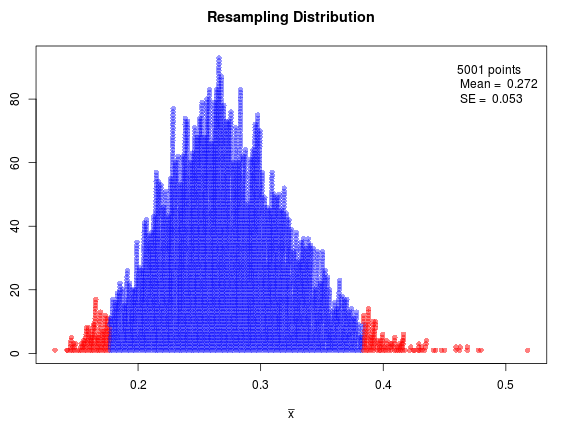
\includegraphics[width=.5\linewidth]{../plots/arsenicCIplot.png}}
\end{key}

Explain how one dot on the plot was created and what it represents in
the context of the problem.
\begin{students}
  \vspace{1cm}
\end{students}
\begin{key}
  {\it One dot was created by sampling with replacement from the
    original data 19 times.  The mean level of arsenic concentration
    in the toenails of the resample is plotted.}
\end{key}

\item \label{SE2ci} Create a 95\% confidence interval using margin of
  error $ME =  2.11  \times SE$.
\begin{students}
  \vspace{1cm}
\end{students}

\begin{key}
  {\it $ 0.272 \pm 2.11(0.053) = (0.16, 0.38)$ ppm}
\end{key}

\item  \label{percentile95} Create a 95\% confidence interval using
  the bootstrap   Percentile Method.
\begin{students}
  \vspace{1cm}
\end{students}

\begin{key}
  {\it $ (0.177, 0.383)$ ppm}
\end{key}

\item  How similar are the confidence intervals in \ref{percentile95}
  and \ref{SE2ci}?
\begin{students}
  \vspace{1cm}
\end{students}

\begin{key}
  {\it Pretty close, the percentile one is a bit higher on both ends
    than the 2.1SE interval.}
\end{key}


\item \label{percentile90}Would you expect a 90\% confidence interval
  to be wider or narrower?  Explain, then give a 90\% (percentile)
  confidence interval.
\begin{students}
  \vspace{2cm}
\end{students}

\begin{key}
  {\it Narrower, we need to capture fewer dots, so we can move in.
    (0.191, 0.365)} 
\end{key}

\item  Interpret the 90\% confidence interval from \ref{percentile90}.
\begin{students}
  \vspace{2cm}
\end{students}

\begin{key}
  {\it We are 90\% confident the true average arsenic level in
    toenails for new Hampshire residents  with a private well is
    between 0.191 and 0.365 ppm. }
\end{key}
\end{enumerate}


{\bf The Second Research Question}: Is the mean arsenic level
for New Hampshire residents with a private well above the 0.15 threshold? 


  There are two possibilities for why the sample average
was 0.272.  List them here and label them as the null and alternative
hypotheses also write the null and alternative in notation.\\
$H_0:$ 
\begin{students}
  \vspace{1cm}
\end{students}
\begin{key}
  {\it   $ \mu = 0.15$:  The water is, on average safe, so we've just
  observed an unusually high sample.}
\end{key}

$H_a:$
\begin{students}
  \vspace{1cm}
\end{students}
\begin{key}

  {\it  $ \mu > 0.15$  The water is, on average, dangerously high in arsenic.}
\end{key}

Is the alternative hypothesis right-tail, left-tail, or two-tail?
\begin{students}
  \vspace{1cm}
\end{students}

\begin{key}
  {\it Right tailed.}
\end{key}

We can simulate the behavior of arsenic concentrations in New
Hampshire ground water if we assume the null hypothesis which gives a
specific value for the mean.  The two key ideas when creating the
reference distribution are:
\begin{itemize}
\item 
 The resamples must be consistent with the null hypothesis.
\item 
 The resamples must be based on the sample data.
\end{itemize}

  We can use cards like we did for the CI above,
but we have to change the values so that they are consistent with the
null, $\mu = 0.15$.

\begin{enumerate}
\setcounter{enumi}{16}
\item How you could modify the sample data so as to force the null
  hypothesis to be true without changing the spread?  (Do not spend
  more than 2 minutes on this question.)
\begin{students}
  \vspace{2cm}
\end{students}

\begin{key}
  {\it  AWV, but if they have read/if you have lectured on this, they
    should know to shift the data to be centered on the null value,
    then resample.} 
\end{key}

% \item Next we will simulate one repetition of the 19 toenail values
%   collected by creating a deck of 19 cards to simulate what the data
%   would look like {\bf if the null hypothesis} were true.
%     \begin{enumerate}
%     \item  What is the null value in this study?
% \begin{students}
%   \vspace{2cm}
% \end{students}

% \begin{key}
%   {\it 0.15}
% \end{key}
\item  \label{shift}How far is the sample mean from this null value?
\begin{students}
  \vspace{2cm}
\end{students}

\begin{key}
  {\it 0.272 – 0.15 = 0.122 above the mean}
\end{key}

\item We need to shift the original data so that is it centered on the null
      value. 
      Subtract the value from (b) from each of the data numbers to
      get:


\begin{center}
\begin{tabular}{|r|r|r|r|r|r|r|r|r|r|} \hline
-0.003 &-0.004 &-0.023 &-0.004 &0.153 &0.236 &-0.042 &0.036 &0.188 &-0.017
\\ \hline
-0.049 &0.710 &0.395 &0.729 &0.147 &0.311 &0.019 &0.013 &0.053
& \\ \hline
\end{tabular}  
\end{center}
      What is the mean of the above values? Why do we want this
      to be the mean?
\begin{students}
  \vspace{1cm}
\end{students}

\begin{key}
  {\it 0.15, because this is the null value. }
\end{key}



\item Now we want to resample the shifted values. To speed up the
  process, we use \fbox{ Test} option under \fbox{One Quant} at
  \webAppURLFrst . You should have already loaded the data, but if
not, go back to \fbox{Input Data} and select the preloaded
\fbox{Arsenic} data.

  \begin{itemize}
    \item Above the main plot, {\bf change the value for the null
      hypothesis} to the one in our null.  (the just barely safe level)
      The software will shift the data to have this mean.
   \end{itemize}

    Look at the box on the left labeled {\sf Original Sample}.
       Does the mean match your answer to \ref{xbar}?  If not, consult
       with your instructor! 
\begin{students}
  \vspace{1cm}
\end{students}

\begin{key}
  {\it Look for data entry errors. }
\end{key}

\item   What is the statistic from the first  resample? (Click the
  blue dot  to see.)
\begin{students}
  \vspace{1cm}
\end{students}

\begin{key}
  {\it AWV}
\end{key}



\item Explain in the context of the problem what the one dot on the
  main plot represents. 
\begin{students}
  \vspace{1cm}
\end{students}

\begin{key}
  {\it The (resample) mean arsenic concentration in toe nails of 19
    New Hampshire residents who use a private well if the true arsenic
    concentration is 0.15 (right at the edge of being  hazardous) }
\end{key}
\item Generate 5000 or more randomization samples.  Copy the summary statistics and
the plot of the randomization distribution below
\begin{students}
  \vspace{4cm}
\end{students}

\begin{key}
  {\it 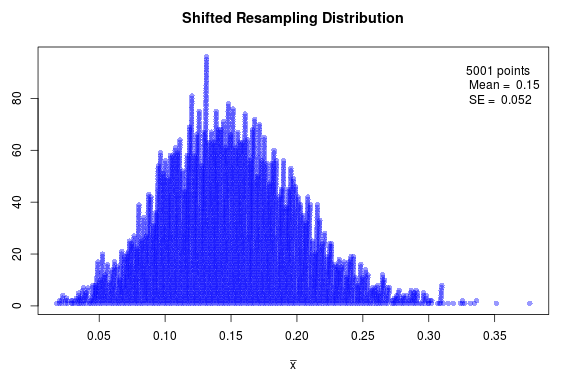
\includegraphics[width=.5\linewidth]{../plots/arsenicNullDistn.png}}
\end{key}


\item 
 Where is the distribution centered?  Why does that make sense?
\begin{students}
  \vspace{1cm}
\end{students}
\begin{key}
  {\it Again, centered at 0.15, because this is the null value. }
\end{key}

Remember why we conducted this simulation: to assess whether the
observed result (mean of 0.272) would be unlikely to occur by chance
alone if the ground water in New Hampshire is not hazardous. 

\item Locate the observed result on the randomization distribution.
  Does it appear to be likely or unlikely to occur under the null
  hypothesis?  Explain your reasoning.
\begin{students}
  \vspace{1cm}
\end{students}

\begin{key}
  {\it Pretty fair in the right tail.  Appears unlikely to occur under
    the null hypothesis. } 
\end{key}

\item \label{pval13}Just how unlikely is the observed result?  Calculate your
  p-value using the web app and the appropriate direction and cutoff value.
\begin{students}
  \vspace{1cm}
\end{students}

\begin{key}
  {\it Right tail p-value = 0.016}
\end{key}

 How many  resamples had a mean at least as extreme as the
 observed result?  
\begin{students}
  \vspace{1cm}
\end{students}

\begin{key}
  {\it AWV}
\end{key}

\item How strong is the evidence against the null hypothesis?  Look back to
  the guidelines for assessing strength of evidence using p-values
  given on page \pageref{fig:SOE-pvalue}.
\begin{students}
  \vspace{1cm}
\end{students}

\begin{key}
  {\it p-value = 0.016, which is strong to very strong evidence
    against the null.}
\end{key}
 

{\bf Step 5: Formulate conclusions.}


\item Based on this analysis, what is your conclusion about the
  residents in New Hampshire who own a private well based on this
  study?
\begin{students}
  \vspace{2cm}
\end{students}

\begin{key}
  {\it We have strong evidence that the true mean arsenic level in
    toenails of NH residents drinking from wells is greater than the
    hazardous threshold of 0.15 ppm.} 
\end{key}
\item Can you extend your results to all of New Hampshire residents?
  All New Hampshire residents with a private well?  Explain your
  reasoning.
\begin{students}
  \vspace{4cm}
\end{students}

\begin{key}
  {\it Our evidence does not extend to all NH residents drinking from
    wells because we don't know that this is a representative sample.
   The data does not include people on municipal water systems, so it
   certainly does not extend to all NH residents.} 
\end{key}

\end{enumerate}

\begin{center}
  {\bf Take Home Messages}\vspace{-.1in}
\end{center}

\begin{itemize}
\item We first reviewed building a CI for a single mean.
\item You need to know when to discuss means versus proportions.  If
  the response has two categories, then we deal with proportions.  If
  the response is quantitative, then we estimate and test means.
\item The new twist today was to do a simulation for testing $H_0: \mu
  = \mu_o$ that the mean is some particular value.  We had to modify
  the data to make $H_0$ true, shifting it from its center at $\xb$ to
  be centered at $\mu_o$.  Then we resampled it as if for a bootstrap
  confidence interval, and located the observed statistic ($\xb$) to
  see how far out in the tails it was (the p--value).

 \item 
Questions? What is your summary of this  lesson? \vfill

\end{itemize}



\noindent
{\bf Assignment} \vspace{-.2in}
\begin{itemize}
 \item D2Quiz 6 is due Oct 13. Fill it in online.
 \item {\bf D2Box 7} is due Oct 17. Turn it in as a pdf file.
 %%  We strongly encourage you to get help in the Math Learning Center.
\item Fill in the simulation confidence interval box in column 2 of
  the Review Table.
\item Watch videos assigned on D2L.
%\item Watch the ``Types of Errors'' video (\# 4 under Unit 2) and Example 8 under Unit 2.
\item Read the next two pages before your next class.
\end{itemize}
